\documentclass[11pt]{article}
\usepackage[margin=1in]{geometry}
\usepackage[T1]{fontenc}
\usepackage{lmodern}
\usepackage{microtype}
\usepackage{amsmath,amssymb}
\usepackage{booktabs}
\usepackage{graphicx}
\usepackage{xcolor}
\usepackage[round]{natbib}
\usepackage[hidelinks]{hyperref}
\usepackage{caption}
\captionsetup{font=small,labelfont=bf}

% Generated by experiments/make_numbers.py. Do not edit.
\newcommand{\NModels}{9}
\newcommand{\NRunsPub}{34}
\newcommand{\NRunsAll}{71}
\newcommand{\NRunsAblation}{56}
\newcommand{\ReproMaxGap}{0.0014}
\newcommand{\ReproMeanGap}{0.0009}
\newcommand{\ReproTau}{0.83}
\newcommand{\ReproTauP}{0.001}
\newcommand{\OverFactor}{2.4}
\newcommand{\PubTableGap}{0.0077}
\newcommand{\MeanRankICPub}{0.0467}
\newcommand{\MeanRankICPost}{0.0198}
\newcommand{\MeanDecayPct}{58\%}
\newcommand{\MinDecayPct}{27\%}
\newcommand{\MaxDecayPct}{79\%}
\newcommand{\MinDecayModel}{LSTM}
\newcommand{\MaxDecayModel}{CatBoost}
\newcommand{\MinPostT}{2.5}
\newcommand{\BestPubModel}{DoubleEnsemble}
\newcommand{\BestPostModel}{LSTM}
\newcommand{\PubLinear}{0.0474}
\newcommand{\PostLinear}{0.0196}
\newcommand{\DecayLinear}{59\%}
\newcommand{\TableLinear}{0.0472}
\newcommand{\PubLightGBM}{0.0483}
\newcommand{\PostLightGBM}{0.0146}
\newcommand{\DecayLightGBM}{70\%}
\newcommand{\TableLightGBM}{0.0469}
\newcommand{\PubXGBoost}{0.0508}
\newcommand{\PostXGBoost}{0.0139}
\newcommand{\DecayXGBoost}{73\%}
\newcommand{\TableXGBoost}{0.0505}
\newcommand{\PubCatBoost}{0.0467}
\newcommand{\PostCatBoost}{0.0097}
\newcommand{\DecayCatBoost}{79\%}
\newcommand{\TableCatBoost}{0.0454}
\newcommand{\PubDoubleEnsemble}{0.0510}
\newcommand{\PostDoubleEnsemble}{0.0153}
\newcommand{\DecayDoubleEnsemble}{70\%}
\newcommand{\TableDoubleEnsemble}{0.0502}
\newcommand{\PubMLP}{0.0439}
\newcommand{\PostMLP}{0.0147}
\newcommand{\DecayMLP}{66\%}
\newcommand{\TableMLP}{0.0429}
\newcommand{\PubGRU}{0.0417}
\newcommand{\PostGRU}{0.0270}
\newcommand{\DecayGRU}{35\%}
\newcommand{\TableGRU}{0.0428}
\newcommand{\PubLSTM}{0.0447}
\newcommand{\PostLSTM}{0.0327}
\newcommand{\DecayLSTM}{27\%}
\newcommand{\TableLSTM}{0.0435}
\newcommand{\PubALSTM}{0.0455}
\newcommand{\PostALSTM}{0.0307}
\newcommand{\DecayALSTM}{33\%}
\newcommand{\TableALSTM}{0.0463}
\newcommand{\BestRecentModel}{Linear}
\newcommand{\BestRecentRankIC}{0.0333}
\newcommand{\RefitShareMin}{22\%}
\newcommand{\RefitShareMax}{80\%}
\newcommand{\MeanRecentStale}{0.0151}
\newcommand{\MeanRecentRefit}{0.0216}
\newcommand{\MeanPubOfRefitted}{0.0469}
\newcommand{\RecentPubLinear}{0.0174}
\newcommand{\RecentRefitLinear}{0.0333}
\newcommand{\RecentRollLinear}{0.0398}
\newcommand{\RefitGainPLinear}{p<0.001}
\newcommand{\RecentPubLightGBM}{0.0113}
\newcommand{\RecentRefitLightGBM}{0.0132}
\newcommand{\RecentRollLightGBM}{0.0152}
\newcommand{\RefitGainPLightGBM}{p=0.411}
\newcommand{\RecentPubXGBoost}{0.0101}
\newcommand{\RecentRefitXGBoost}{0.0161}
\newcommand{\RecentRollXGBoost}{0.0175}
\newcommand{\RefitGainPXGBoost}{p=0.089}
\newcommand{\RecentPubCatBoost}{0.0042}
\newcommand{\RecentRefitCatBoost}{0.0104}
\newcommand{\RefitGainPCatBoost}{p=0.094}
\newcommand{\RecentPubDoubleEnsemble}{0.0119}
\newcommand{\RecentRefitDoubleEnsemble}{0.0178}
\newcommand{\RefitGainPDoubleEnsemble}{p=0.090}
\newcommand{\RecentPubMLP}{0.0108}
\newcommand{\RecentRefitMLP}{0.0163}
\newcommand{\RefitGainPMLP}{p=0.061}
\newcommand{\RecentPubGRU}{0.0256}
\newcommand{\RecentRefitGRU}{0.0333}
\newcommand{\RefitGainPGRU}{p=0.139}
\newcommand{\RecentPubLSTM}{0.0316}
\newcommand{\RecentPubALSTM}{0.0298}
\newcommand{\RecentRefitALSTM}{0.0324}
\newcommand{\RefitGainPALSTM}{p=0.754}
\newcommand{\DaysPub}{871}
\newcommand{\MCSSizePub}{6}
\newcommand{\MCSOfPub}{9}
\newcommand{\MCSListPub}{Linear, LightGBM, XGBoost, DoubleEnsemble, LSTM, ALSTM}
\newcommand{\PairsPub}{36}
\newcommand{\PairsSigPub}{10}
\newcommand{\PairsHolmPub}{1}
\newcommand{\MedianSEPub}{0.0045}
\newcommand{\SPALightGBMPub}{p=0.21}
\newcommand{\SPALinearPub}{p=0.12}
\newcommand{\DaysPost}{1521}
\newcommand{\MCSSizePost}{2}
\newcommand{\MCSOfPost}{9}
\newcommand{\MCSListPost}{LSTM, ALSTM}
\newcommand{\PairsPost}{36}
\newcommand{\PairsSigPost}{25}
\newcommand{\PairsHolmPost}{21}
\newcommand{\MedianSEPost}{0.0035}
\newcommand{\SPALightGBMPost}{p<0.01}
\newcommand{\SPALinearPost}{p<0.01}
\newcommand{\DaysRecent}{933}
\newcommand{\MCSSizeRecent}{3}
\newcommand{\MCSOfRecent}{8}
\newcommand{\MCSListRecent}{Linear, GRU, ALSTM}
\newcommand{\PairsRecent}{28}
\newcommand{\PairsSigRecent}{18}
\newcommand{\PairsHolmRecent}{15}
\newcommand{\MedianSERecent}{0.0046}
\newcommand{\SPALightGBMRecent}{p<0.01}
\newcommand{\SPALinearRecent}{p=0.67}
\newcommand{\ICCPub}{0.75}
\newcommand{\SeedSDPub}{0.0019}
\newcommand{\ModelSDPub}{0.0032}
\newcommand{\ICCPost}{0.96}
\newcommand{\SeedSDPost}{0.0015}
\newcommand{\ModelSDPost}{0.0077}
\newcommand{\ICCRecent}{0.77}
\newcommand{\SeedSDRecent}{0.0016}
\newcommand{\ModelSDRecent}{0.0029}
\newcommand{\TauPubPost}{-0.33}
\newcommand{\TauPPubPost}{0.26}
\newcommand{\TauTablePost}{-0.28}
\newcommand{\TauPTablePost}{0.36}
\newcommand{\TauPubRecent}{-0.14}
\newcommand{\TauPPubRecent}{0.72}
\newcommand{\TauTableRecent}{-0.07}
\newcommand{\TauPTableRecent}{0.90}
\newcommand{\KeptRankMin}{41\%}
\newcommand{\KeptRankMax}{73\%}
\newcommand{\KeptZMin}{21\%}
\newcommand{\KeptZMax}{34\%}
\newcommand{\NRankModels}{4}
\newcommand{\NZModels}{5}
\newcommand{\AblLGBRankPost}{0.0286}
\newcommand{\AblLGBRankPub}{0.0553}
\newcommand{\AblLGBRankRecent}{0.0295}
\newcommand{\AblLGBRankPostIC}{0.0201}
\newcommand{\AblBaseLGBRankPost}{0.0146}
\newcommand{\AblBaseLGBRankPub}{0.0483}
\newcommand{\AblBaseLGBRankRecent}{0.0132}
\newcommand{\AblBaseLGBRankPostIC}{0.0179}
\newcommand{\AblLGBRankRatio}{2.0}
\newcommand{\AblLGBRankGain}{0.0140}
\newcommand{\AblLGBRankP}{p<0.001}
\newcommand{\AblXGBRankPost}{0.0281}
\newcommand{\AblXGBRankPub}{0.0568}
\newcommand{\AblXGBRankRecent}{0.0336}
\newcommand{\AblXGBRankPostIC}{0.0212}
\newcommand{\AblBaseXGBRankPost}{0.0139}
\newcommand{\AblBaseXGBRankPub}{0.0508}
\newcommand{\AblBaseXGBRankRecent}{0.0161}
\newcommand{\AblBaseXGBRankPostIC}{0.0183}
\newcommand{\AblXGBRankRatio}{2.0}
\newcommand{\AblXGBRankGain}{0.0142}
\newcommand{\AblXGBRankP}{p<0.001}
\newcommand{\AblCatRankPost}{0.0291}
\newcommand{\AblCatRankPub}{0.0574}
\newcommand{\AblCatRankRecent}{0.0336}
\newcommand{\AblCatRankPostIC}{0.0221}
\newcommand{\AblBaseCatRankPost}{0.0097}
\newcommand{\AblBaseCatRankPub}{0.0467}
\newcommand{\AblBaseCatRankRecent}{0.0104}
\newcommand{\AblBaseCatRankPostIC}{0.0172}
\newcommand{\AblCatRankRatio}{3.0}
\newcommand{\AblCatRankGain}{0.0194}
\newcommand{\AblCatRankP}{p<0.001}
\newcommand{\AblDERankPost}{0.0298}
\newcommand{\AblDERankPub}{0.0559}
\newcommand{\AblDERankRecent}{0.0364}
\newcommand{\AblDERankPostIC}{0.0217}
\newcommand{\AblBaseDERankPost}{0.0153}
\newcommand{\AblBaseDERankPub}{0.0510}
\newcommand{\AblBaseDERankRecent}{0.0178}
\newcommand{\AblBaseDERankPostIC}{0.0194}
\newcommand{\AblDERankRatio}{1.9}
\newcommand{\AblDERankGain}{0.0145}
\newcommand{\AblDERankP}{p<0.001}
\newcommand{\AblMLPRankPost}{0.0218}
\newcommand{\AblMLPRankPub}{0.0480}
\newcommand{\AblMLPRankRecent}{0.0247}
\newcommand{\AblMLPRankPostIC}{0.0165}
\newcommand{\AblBaseMLPRankPost}{0.0147}
\newcommand{\AblBaseMLPRankPub}{0.0439}
\newcommand{\AblBaseMLPRankRecent}{0.0163}
\newcommand{\AblBaseMLPRankPostIC}{0.0170}
\newcommand{\AblMLPRankRatio}{1.5}
\newcommand{\AblMLPRankGain}{0.0071}
\newcommand{\AblMLPRankP}{p<0.001}
\newcommand{\AblLinearZPost}{0.0100}
\newcommand{\AblLinearZPub}{0.0410}
\newcommand{\AblLinearZRecent}{0.0191}
\newcommand{\AblLinearZPostIC}{0.0157}
\newcommand{\AblBaseLinearZPost}{0.0196}
\newcommand{\AblBaseLinearZPub}{0.0474}
\newcommand{\AblBaseLinearZRecent}{0.0333}
\newcommand{\AblBaseLinearZPostIC}{0.0162}
\newcommand{\AblLinearZRatio}{0.5}
\newcommand{\AblLinearZGain}{-0.0097}
\newcommand{\AblLinearZP}{p<0.001}
\newcommand{\AblLGBTwentyPost}{0.0055}
\newcommand{\AblLGBTwentyPub}{0.0322}
\newcommand{\AblLGBTwentyRecent}{0.0056}
\newcommand{\AblLGBTwentyPostIC}{0.0123}
\newcommand{\AblBaseLGBTwentyPost}{0.0146}
\newcommand{\AblBaseLGBTwentyPub}{0.0483}
\newcommand{\AblBaseLGBTwentyRecent}{0.0132}
\newcommand{\AblBaseLGBTwentyPostIC}{0.0179}
\newcommand{\AblLGBTwentyRatio}{0.4}
\newcommand{\AblLGBTwentyGain}{-0.0091}
\newcommand{\AblLGBTwentyP}{p<0.001}
\newcommand{\PredHeld}{all four}
\newcommand{\PredOne}{held}
\newcommand{\PredTwo}{held}
\newcommand{\PredThree}{held}
\newcommand{\PredFour}{held}
\newcommand{\FeatN}{158}
\newcommand{\FeatStrong}{138}
\newcommand{\FeatTrain}{0.0275}
\newcommand{\FeatPub}{0.0120}
\newcommand{\FeatPost}{0.0060}
\newcommand{\FeatDropTrainPub}{56\%}
\newcommand{\FeatDropPubPost}{50\%}
\newcommand{\FeatSlope}{0.67}
\newcommand{\FeatFlips}{18}
\newcommand{\FeatMedianRatio}{0.58}
\newcommand{\RetPubALSTM}{5.8\%}
\newcommand{\IRPubALSTM}{0.92}
\newcommand{\RetPostALSTM}{5.8\%}
\newcommand{\IRPostALSTM}{0.74}
\newcommand{\RetPubCatBoost}{8.9\%}
\newcommand{\IRPubCatBoost}{0.95}
\newcommand{\RetPostCatBoost}{4.6\%}
\newcommand{\IRPostCatBoost}{0.40}
\newcommand{\RetPubDoubleEnsemble}{11.5\%}
\newcommand{\IRPubDoubleEnsemble}{1.33}
\newcommand{\RetPostDoubleEnsemble}{5.1\%}
\newcommand{\IRPostDoubleEnsemble}{0.51}
\newcommand{\RetPubGRU}{5.0\%}
\newcommand{\IRPubGRU}{0.70}
\newcommand{\RetPostGRU}{6.9\%}
\newcommand{\IRPostGRU}{0.86}
\newcommand{\RetPubLightGBM}{12.4\%}
\newcommand{\IRPubLightGBM}{1.41}
\newcommand{\RetPostLightGBM}{2.2\%}
\newcommand{\IRPostLightGBM}{0.21}
\newcommand{\RetPubLinear}{9.9\%}
\newcommand{\IRPubLinear}{1.31}
\newcommand{\RetPostLinear}{5.8\%}
\newcommand{\IRPostLinear}{0.69}
\newcommand{\RetPubLSTM}{3.8\%}
\newcommand{\IRPubLSTM}{0.56}
\newcommand{\RetPostLSTM}{7.8\%}
\newcommand{\IRPostLSTM}{1.01}
\newcommand{\RetPubMLP}{5.6\%}
\newcommand{\IRPubMLP}{0.73}
\newcommand{\RetPostMLP}{6.7\%}
\newcommand{\IRPostMLP}{0.78}
\newcommand{\RetPubXGBoost}{9.4\%}
\newcommand{\IRPubXGBoost}{1.01}
\newcommand{\RetPostXGBoost}{4.2\%}
\newcommand{\IRPostXGBoost}{0.37}
\newcommand{\RetRecentALSTM}{4.2\%}
\newcommand{\IRRecentALSTM}{0.54}
\newcommand{\RetRecentCatBoost}{7.8\%}
\newcommand{\IRRecentCatBoost}{0.75}
\newcommand{\RetRecentDoubleEnsemble}{8.1\%}
\newcommand{\IRRecentDoubleEnsemble}{0.91}
\newcommand{\RetRecentGRU}{-0.0\%}
\newcommand{\IRRecentGRU}{-0.00}
\newcommand{\RetRecentLightGBM}{4.1\%}
\newcommand{\IRRecentLightGBM}{0.43}
\newcommand{\RetRecentLinear}{7.3\%}
\newcommand{\IRRecentLinear}{0.82}
\newcommand{\RetRecentMLP}{7.9\%}
\newcommand{\IRRecentMLP}{0.92}
\newcommand{\RetRecentXGBoost}{7.3\%}
\newcommand{\IRRecentXGBoost}{0.76}
\newcommand{\MeanRetPub}{8.0\%}
\newcommand{\MeanRetPost}{5.5\%}
\newcommand{\NullRetPub}{-8.8\%}
\newcommand{\NullRetSDPub}{0.7\%}
\newcommand{\NullIRPub}{-1.30}
\newcommand{\NullRetPost}{-0.9\%}
\newcommand{\NullRetSDPost}{2.3\%}
\newcommand{\NullIRPost}{-0.14}
\newcommand{\NullRetRecent}{-0.9\%}
\newcommand{\NullRetSDRecent}{3.5\%}
\newcommand{\NullIRRecent}{-0.15}
\newcommand{\AboveNullPub}{16.8\%}
\newcommand{\AboveNullPost}{6.4\%}
\newcommand{\AboveNullDrop}{62\%}
\newcommand{\RetLGBRankPost}{5.1\%}
\newcommand{\RetLGBRankRecent}{5.1\%}
\newcommand{\RetXGBRankPost}{7.2\%}
\newcommand{\RetXGBRankRecent}{5.6\%}
\newcommand{\RetCatRankPost}{8.7\%}
\newcommand{\RetCatRankRecent}{6.9\%}
\newcommand{\RetDERankPost}{7.5\%}
\newcommand{\RetDERankRecent}{9.3\%}
\newcommand{\RetMLPRankPost}{5.3\%}
\newcommand{\RetMLPRankRecent}{4.9\%}
\newcommand{\RetLinearZPost}{4.6\%}
\newcommand{\RetLinearZRecent}{6.6\%}
\newcommand{\RankBetterRetPost}{4}
\newcommand{\RankBetterRetRecent}{2}
\newcommand{\RankBetterRetOf}{5}
\newcommand{\DSRBest}{LSTM (seed 0)}
\newcommand{\DSRTrials}{33}
\newcommand{\DSRIR}{0.90}
\newcommand{\DSRValue}{0.88}
\newcommand{\DSRPSR}{0.989}
\newcommand{\DSRSRZero}{0.45}


\title{What Survives Out of Sample?\\[2pt]
\large A Post-Publication Audit of the Qlib Stock-Prediction Benchmark on Chinese A-Shares}
\author{Le Nam Khanh\\[2pt]
\small The Hong Kong Polytechnic University}
\date{November 2026}

\begin{document}
\maketitle

\begin{abstract}
The Alpha158 / CSI\,300 leaderboard of Microsoft's Qlib platform is a common yardstick for machine-learning models of Chinese stock returns, and recent papers still report against it.
Every number on it comes from one test window, January 2017 to July 2020.
We re-run the official configurations of \NModels{} of its models, unchanged except for the data source and the time segments, in \NRunsAll{} training runs (and \NRunsAblation{} more for ablations), on independently maintained daily data that include delisted stocks and run to 13 November 2026.
Inside the published window the leaderboard reproduces closely: every model's mean daily Rank IC lies within \ReproMaxGap{} of the published value.
In the six years after it, the mean Rank IC across models falls from \MeanRankICPub{} to \MeanRankICPost{}, a decline of \MeanDecayPct{}, and the benchmark portfolio's excess return over a random-score strategy falls by \AboveNullDrop{}.
The ranking does not carry over: the differences between models exceed seed noise in every window, but the Kendall correlation between the rankings before and after July 2020 is $\tau=\TauPubPost$.
The models that held up are the ones whose configuration trains on a cross-sectionally ranked label rather than a z-scored one, and a single-change ablation confirms it: switching LightGBM's label from z-scores to ranks multiplies its post-2020 Rank IC by \AblLGBRankRatio{}, a change larger than the published gap between any two of the nine models.
A feature-level analysis shows that the decay began before the benchmark window and continued after it.
Single-window leaderboards in this domain should be read as in-sample results, and comparisons between model families as comparisons between whole configurations; we release the full pipeline.
\end{abstract}

\section{Introduction}

Qlib \citep{yang2020qlib} made it easy to train and compare stock-return models on a common data set, feature set and backtest.
Its benchmark table for the CSI\,300 universe with the Alpha158 features lists more than fifteen models, from ordinary least squares to gradient-boosted trees, recurrent networks and Transformers, each with the mean and standard deviation over twenty seeds of four signal metrics and three portfolio metrics.
New methods are still compared against these baselines on the same test window \citep[e.g.][]{lin2025cspo}, and the model zoo is used as a set of reference strategies for newer systems, including LLM trading agents \citep{zhu2026ktdfin}.

Every number in the table is computed on one window, 1 January 2017 to 1 August 2020.
That window is now six years old.
Finance has a long record of predictors that weaken once they are published or simply once the sample moves on \citep{mclean2016does,falck2022decay,harvey2016cross,jensen2023replication}, and machine-learning benchmarks have their own record of rankings that do not survive a change of seed \citep{henderson2018deep,bouthillier2021accounting}.
This paper asks what the Qlib leaderboard says about the six years that followed it.
We ask four questions.

\begin{enumerate}
\item \textbf{Reproduction.} With independent data, do the official configurations reproduce the published numbers on the published window?
\item \textbf{Decay.} How much predictive power is left after July 2020, and is the loss a matter of stale models or of a changed market?
\item \textbf{Ranking.} Are the differences between models larger than the noise from random seeds and from the finite test window, before and after 2020?
\item \textbf{Value.} What is left of the portfolio performance once transaction costs and the number of models tried are taken into account?
\end{enumerate}

Our contribution is an audit, not a new model.
We re-execute the official configuration files of \NModels{} models with several seeds each (\S\ref{sec:setup}); we extend their test segment by six years, refit them on a later window and, for three cheap models, refit them every year (\S\ref{sec:protocols}); and we read the results with tests that account for serial correlation and for the number of models compared (\S\ref{sec:inference}).
In brief (\S\ref{sec:results}):
(1) inside the published window the table reproduces on independent data;
(2) after it, about \MeanDecayPct{} of the average Rank IC is gone, and refitting on later data recovers only part of it;
(3) the differences between models are larger than seed noise in every window, but their order does not carry over;
(4) the configurations that held up are the ones that train on a ranked label, and changing only the label of the others moves them by more than the published gap between any two of these models;
(5) the decline of the underlying features started before the published window.
\S\ref{sec:discussion} discusses what these results do and do not imply.

\section{Data, models and deviations}\label{sec:setup}

\paragraph{Data.}
We use the daily A-share database that the open-source project \texttt{investment\_data} distributes in Qlib's binary format \citep{chendi2026data}, release of 14 November 2026 (SHA-256 of the archive recorded in the repository).
It is merged from several sources with cross-source validation, covers 6{,}176 listings from 4 January 2000 to 13 November 2026, keeps delisted stocks, and stores the constituents of the CSI\,300 index as dated membership intervals, so that the universe on each date is the index as it was on that date.
The data used for the published table were collected by Qlib's own scripts from a different source; we therefore expect close, not exact, agreement.

\paragraph{Features and label.}
Features are the 158 Alpha158 expressions computed by Qlib's own handler; the label is Qlib's default, $y_{i,t}=P_{i,t+2}/P_{i,t+1}-1$ on adjusted closing prices, the return from the close after the signal date to the close one day later.
The universe is the CSI\,300 on each date.
We compute features and labels once for 2008--2026 and cache them; each run then applies the processors of its own configuration, fitted on its own training window.

\paragraph{Models.}
We use the official configuration files of Qlib at commit \texttt{54355232} for Linear (OLS), LightGBM \citep{ke2017lightgbm}, XGBoost \citep{chen2016xgboost}, CatBoost \citep{prokhorenkova2018catboost}, DoubleEnsemble \citep{zhang2020doubleensemble}, a multilayer perceptron, GRU \citep{cho2014learning}, LSTM \citep{hochreiter1997long} and ALSTM \citep{qin2017dual}; the recurrent models use the twenty Alpha158 features selected in the official configurations.
Hyperparameters, processors, early stopping and losses are exactly those of the files.
One difference between the files matters later: before training, the configurations of Linear and of the recurrent models replace each day's labels by their cross-sectional ranks (\texttt{CSRankNorm}), while those of the tree models and the MLP standardise them to z-scores (\texttt{CSZScoreNorm}), which keeps the heavy tails of daily returns in the training target.

\paragraph{Deviations.}
Everything that differs from the official workflow is listed here.
(i) The data source, above.
(ii) The test segment runs to the end of the data instead of stopping at 1 August 2020; the fitted models are identical.
(iii) Seeds: under the published protocol we run five seeds for the tree models and the MLP, three for GRU and ALSTM and two for LSTM, against twenty in the published table; under the refit protocol, five for the tree models and the MLP and one for GRU and ALSTM. The published tree results show a standard deviation of zero because they were not seeded, while ours vary the column and row subsampling.
(iv) Hardware: thread counts are capped at the two CPU cores we used, and CatBoost's Poisson bootstrap, which exists only on GPUs, is replaced by Bernoulli subsampling at the same rate.
(v) Qlib's cross-sectional mean-fill processor is replaced by a vectorised version with identical output (difference below $10^{-15}$, checked by a test), because the original needs more than the 8\,GB of memory available.
(vi) A one-line shim lets Qlib's MLP pass a logging argument that current PyTorch no longer accepts.

\section{Protocols}\label{sec:protocols}

\begin{table}[t]
\centering\small
\caption{Training protocols. Segments are inclusive; processors are fitted on the training segment.}\label{tab:protocols}
\begin{tabular}{llll}
\toprule
Protocol & Train & Validation & Test \\
\midrule
Published & 2008--2014 & 2015--2016 & 2017-01-01 to 2026-11-13 \\
Refit & 2014--2020 & 2021--2022 & 2023-01-01 to 2026-11-13 \\
Annual refit & $[Y-9,\,Y-3]$ & $[Y-2,\,Y-1]$ & year $Y=2017,\dots,2026$ \\
\bottomrule
\end{tabular}
\end{table}

Table~\ref{tab:protocols} lists the three protocols.
The \emph{published} protocol is the official one with a longer test segment; it lets us score exactly the published models on three windows: the \emph{published window} (2017-01-01 to 2020-07-31, \DaysPub{} trading days), the \emph{post window} (2020-08-01 to 2026-11-13, \DaysPost{} days with a label) and the \emph{recent window} (2023-01-01 onwards, \DaysRecent{} days).
The \emph{refit} protocol moves all segments six years forward, so that its test segment starts right after its validation segment, as the published one did in 2017.
Comparing the published and refit protocols on the recent window separates staleness from everything else.
The \emph{annual refit} protocol, run for Linear and the two cheapest tree models, retrains every year on a sliding window of the same lengths.

\section{Measurement and inference}\label{sec:inference}

\paragraph{Signal metrics.}
On each day $t$, the IC is the Pearson correlation and the Rank IC the Spearman correlation between the model score and $y_{i,t}$ across the stocks in the universe; ICIR is the mean daily IC over its standard deviation.
These are Qlib's definitions.
We report each metric as the mean over seeds of the per-seed value, and use the \emph{seed ensemble}, the average of the per-day standardised scores of all seeds, when a test needs one daily series per model.

\paragraph{Serial correlation.}
Daily ICs are autocorrelated because scores and holdings change slowly.
Standard errors of means use the Newey--West estimator with Bartlett weights and $\lfloor 4(T/100)^{2/9}\rfloor$ lags \citep{newey1987simple,newey1994automatic}.
Two models are compared on the same days through the paired difference $d_t=\mathrm{RankIC}_{A,t}-\mathrm{RankIC}_{B,t}$, whose mean is divided by its own HAC standard error, a Diebold--Mariano test \citep{diebold1995comparing}.

\paragraph{Many models at once.}
The model confidence set (MCS) of \citet{hansen2011mcs} is the set of models that cannot be rejected as best at the 10\% level; we use the loss $-\mathrm{RankIC}_{m,t}$, the range statistic, and 2{,}000 stationary-bootstrap replications with mean block length 10 \citep{politis1994stationary}.
Hansen's test of superior predictive ability \citep[SPA,][]{hansen2005spa} asks whether any model beats a given benchmark; we report its consistent p-value against LightGBM and against Linear.

\paragraph{Seed noise.}
For each window, let $\bar r_{ms}$ be the mean daily Rank IC of model $m$ trained with seed $s$.
A one-way random-effects decomposition of $\{\bar r_{ms}\}$ gives a between-model variance $\sigma^2_{\text{model}}$ and a within-model (seed) variance $\sigma^2_{\text{seed}}$; their ratio $\sigma^2_{\text{model}}/(\sigma^2_{\text{model}}+\sigma^2_{\text{seed}})$ is the share of run-to-run variation explained by the choice of model.

\paragraph{Portfolios.}
We use Qlib's own backtest with the benchmark settings: hold the 50 highest-scored stocks, replace at most 5 per day, trade at the close with 5 basis points to buy and 15 to sell (minimum 5 yuan), forbid trades in stocks that moved more than 9.5\%, and start with $10^8$ yuan.
The daily excess return is the portfolio return minus the CSI\,300 return minus costs.
Following Qlib, annualised excess return is $238$ times the daily mean and the information ratio is the daily mean over its standard deviation times $\sqrt{238}$.
For the best strategy after 2020 we report the deflated Sharpe ratio \citep{bailey2014deflated}, the probability that its true Sharpe ratio exceeds the maximum expected from the number of strategies tried when none has skill, computed from the probabilistic Sharpe ratio \citep{bailey2012sharpe}.

\section{Results}\label{sec:results}

\subsection{The leaderboard reproduces}

\begin{table}[t]
\centering\small
\caption{Published window (2017-01-01 to 2020-07-31). Published values are from the Qlib table (mean of twenty seeds); ours are means over our seeds ($\pm$ one standard deviation across seeds for Rank IC). Annualised excess return in percent.}\label{tab:repro}
\setlength{\tabcolsep}{4pt}
\begin{tabular}{lrrrrrrrrr}
\toprule
 & & \multicolumn{2}{c}{IC} & \multicolumn{2}{c}{Rank IC} & \multicolumn{2}{c}{Excess return} & \multicolumn{2}{c}{Inf.\ ratio} \\
\cmidrule(lr){3-4}\cmidrule(lr){5-6}\cmidrule(lr){7-8}\cmidrule(lr){9-10}
Model & Seeds & Publ. & Ours & Publ. & Ours & Publ. & Ours & Publ. & Ours \\
\midrule
Linear & 1 & 0.0397 & 0.0392 & 0.0472 & 0.0474 & 6.9 & 9.9 & 0.92 & 1.31 \\
LightGBM & 5 & 0.0448 & 0.0460 & 0.0469 & 0.0483\,$\pm$\,0.0018 & 9.0 & 11.1 & 1.02 & 1.25 \\
XGBoost & 5 & 0.0498 & 0.0597 & 0.0505 & 0.0508\,$\pm$\,0.0012 & 7.8 & 10.9 & 0.91 & 1.21 \\
CatBoost & 5 & 0.0481 & 0.0561 & 0.0454 & 0.0467\,$\pm$\,0.0013 & 7.6 & 9.3 & 0.80 & 1.01 \\
DoubleEnsemble & 5 & 0.0521 & 0.0532 & 0.0502 & 0.0510\,$\pm$\,0.0003 & 11.6 & 11.2 & 1.34 & 1.28 \\
MLP & 5 & 0.0376 & 0.0423 & 0.0429 & 0.0439\,$\pm$\,0.0020 & 8.9 & 7.2 & 1.14 & 0.94 \\
GRU & 3 & 0.0315 & 0.0317 & 0.0428 & 0.0417\,$\pm$\,0.0044 & 3.4 & 3.4 & 0.52 & 0.49 \\
LSTM & 2 & 0.0318 & 0.0322 & 0.0435 & 0.0447\,$\pm$\,0.0015 & 3.8 & 2.2 & 0.56 & 0.34 \\
ALSTM & 3 & 0.0362 & 0.0312 & 0.0463 & 0.0455\,$\pm$\,0.0011 & 4.7 & 5.0 & 0.70 & 0.76 \\
\bottomrule

\end{tabular}
\end{table}

Table~\ref{tab:repro} compares our runs with the published table on the published window.
The mean absolute gap in Rank IC is \ReproMeanGap{} and the largest is \ReproMaxGap{}; the rankings by Rank IC agree with Kendall $\tau=\ReproTau$ (exact $p=\ReproTauP$).
Our ICs are somewhat higher than the published ones for the tree models, which we attribute to the cleaner data, but the leaderboard's shape is intact: the boosted trees lead, and the published leader, DoubleEnsemble, is again at or near the top.
The portfolio metrics reproduce less exactly, as expected for a strategy that turns over a few stocks a day, but the order of magnitude and the ranking are similar.
This matters for everything that follows: the declines below are not an artefact of a broken pipeline.

\subsection{Six years later, most of the signal is gone}

\begin{figure}[t]
\centering
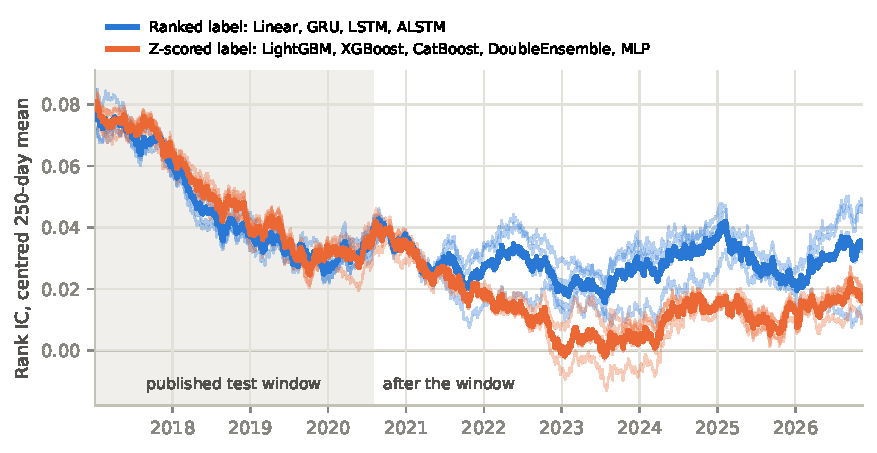
\includegraphics[width=\linewidth]{figures/rolling_rank_ic.pdf}
\caption{Centred 250-day mean of the daily Rank IC under the published protocol. Thin lines: each model's seed ensemble; thick lines: the mean of each group. Blue: configurations that train on a cross-sectionally ranked label; orange: on a z-scored label. The shaded band is the published test window.}\label{fig:rolling}
\end{figure}

\begin{table}[t]
\centering\small
\caption{Mean daily Rank IC by window. ``Change'' compares the post window with the published window under the published protocol; $t$ is the Newey--West $t$-statistic of the post-window mean of the seed ensemble. The last three columns score the recent window (2023--2026) with the published models, with models refitted on 2014--2020, and with annual refits.}\label{tab:decay}
\setlength{\tabcolsep}{5pt}
\begin{tabular}{lrrrrrrr}
\toprule
 & \multicolumn{4}{c}{Published protocol} & \multicolumn{3}{c}{Recent window, 2023--2026} \\
\cmidrule(lr){2-5}\cmidrule(lr){6-8}
Model & 2017--07/2020 & 08/2020--2026 & Change & $t$ & Published & Refit & Annual \\
\midrule
Linear & 0.0474 & 0.0196 & -59\% & 5.3 & 0.0174 & 0.0333 & 0.0398 \\
LightGBM & 0.0483 & 0.0146 & -70\% & 4.5 & 0.0113 & 0.0132 & 0.0152 \\
XGBoost & 0.0508 & 0.0139 & -73\% & 4.1 & 0.0101 & 0.0161 & 0.0175 \\
CatBoost & 0.0467 & 0.0097 & -79\% & 2.5 & 0.0042 & 0.0104 & -- \\
DoubleEnsemble & 0.0510 & 0.0153 & -70\% & 4.7 & 0.0119 & 0.0178 & -- \\
MLP & 0.0439 & 0.0147 & -66\% & 4.4 & 0.0108 & 0.0163 & -- \\
GRU & 0.0417 & 0.0270 & -35\% & 8.5 & 0.0256 & 0.0333 & -- \\
LSTM & 0.0447 & 0.0327 & -27\% & 10.3 & 0.0316 & -- & -- \\
ALSTM & 0.0455 & 0.0307 & -33\% & 9.4 & 0.0298 & 0.0324 & -- \\
\bottomrule

\end{tabular}
\end{table}

Figure~\ref{fig:rolling} and Table~\ref{tab:decay} show what happened next.
Averaged over models, the Rank IC falls from \MeanRankICPub{} in the published window to \MeanRankICPost{} after it, a decline of \MeanDecayPct{}; the decline ranges from \MinDecayPct{} (\MinDecayModel) to \MaxDecayPct{} (\MaxDecayModel).
The signal does not vanish: every model keeps a positive post-window Rank IC with a Newey--West $t$ of at least \MinPostT{}.
A reader who took the published table as an estimate of future performance would, on average, have overestimated it by a factor of \OverFactor{}.

Is this staleness?
The published models were fitted on data that ended in 2016.
Refitting on 2014--2020 and testing on 2023--2026 (Table~\ref{tab:decay}, last columns) raises the average Rank IC on that window from \MeanRecentStale{} to \MeanRecentRefit{}, against \MeanPubOfRefitted{} for the same models in the published window.
The gain is large for Linear (\RecentPubLinear{} to \RecentRefitLinear{}, paired $\RefitGainPLinear$) and small for the tree models (LightGBM \RecentPubLightGBM{} to \RecentRefitLightGBM{}, $\RefitGainPLightGBM$); refitted models reach between \RefitShareMin{} and \RefitShareMax{} of their published-window level, and annual retraining does not bring the tree models back either.
Most of the loss therefore belongs to the market, not to the age of the models.

\subsection{The ranking does not survive}

\begin{figure}[t]
\centering
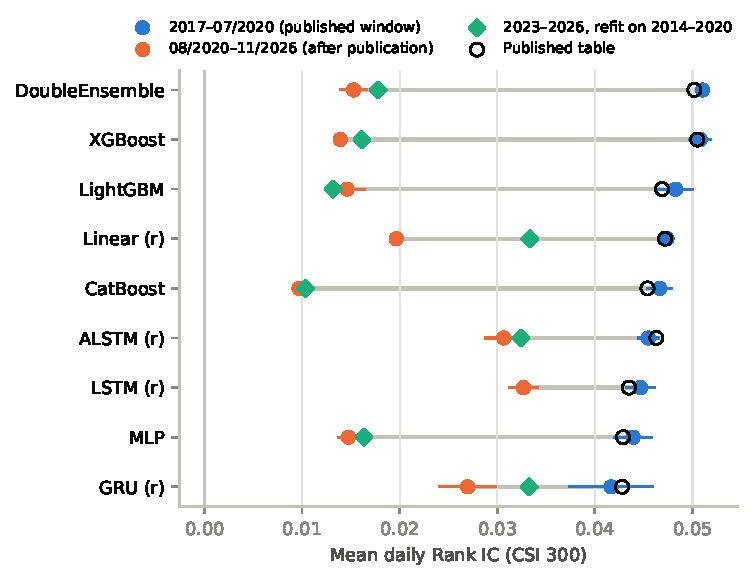
\includegraphics[width=0.78\linewidth]{figures/dumbbell.pdf}
\caption{Mean daily Rank IC of each model in the published window (blue) and after it (orange) under the published protocol, refitted on 2014--2020 and tested on 2023--2026 (diamonds), and as published by Qlib (circles). Bars span one standard deviation across seeds.}\label{fig:dumbbell}
\end{figure}

\begin{figure}[t]
\centering
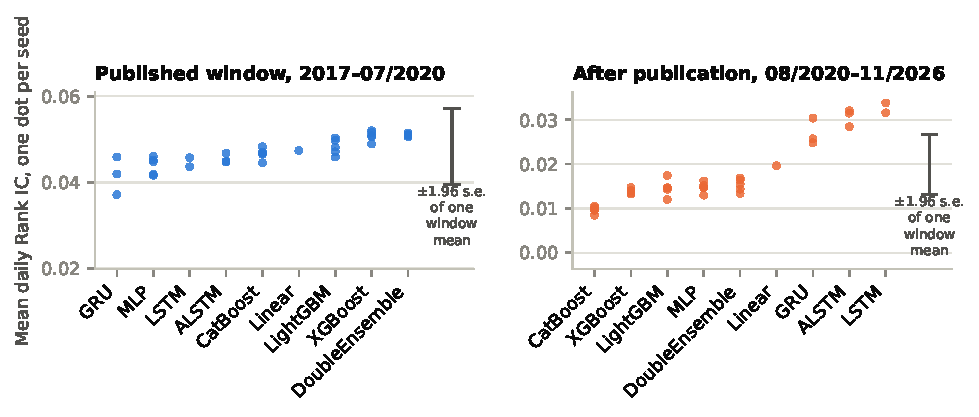
\includegraphics[width=\linewidth]{figures/seed_noise.pdf}
\caption{Mean daily Rank IC of every (model, seed) run. The shaded band is $\pm1.96$ times the median Newey--West standard error of one model's mean over the window: the sampling error of the test window alone.}\label{fig:seeds}
\end{figure}

\begin{table}[t]
\centering\small
\caption{Is the ranking real? MCS: models in the 90\% model confidence set. Pairs: pairwise paired tests with $p<0.05$, and the number that survive Holm's correction. SPA: consistent p-values of Hansen's test that some model beats LightGBM or Linear. Model share: $\sigma^2_{\text{model}}/(\sigma^2_{\text{model}}+\sigma^2_{\text{seed}})$.}\label{tab:tests}
\setlength{\tabcolsep}{5pt}
\begin{tabular}{lrrrrrrr}
\toprule
Window & Days & MCS & Pairs & Holm & SPA vs LGBM & SPA vs Linear & Model share \\
\midrule
2017--07/2020 & 871 & 6/9 & 10/36 & 1 & 0.21 & 0.12 & 0.75 \\
08/2020--11/2026 & 1521 & 2/9 & 25/36 & 21 & 0.00 & 0.00 & 0.96 \\
2023--2026 (refit) & 933 & 3/8 & 18/28 & 15 & 0.00 & 0.67 & 0.77 \\
\bottomrule

\end{tabular}
\end{table}

A leaderboard is useful if its order carries over.
Inside the published window, ours does: the Kendall correlation between the published table and our published-window ranking is \ReproTau{}.
After the window it does not.
The correlation between our published-window ranking and the post-window ranking is $\tau=\TauPubPost$ ($p=\TauPPubPost$), and between the published table and the post-window ranking $\tau=\TauTablePost$ (Figure~\ref{fig:dumbbell}).
The best model in the published window is \BestPubModel; after it, \BestPostModel.

Is the reshuffling just noise?
Two kinds of noise matter, and they point in different directions (Table~\ref{tab:tests}, Figure~\ref{fig:seeds}).
\emph{Seed noise is small.}
In every window the choice of model explains most of the variation between training runs: the model share is \ICCPub{} in the published window, \ICCPost{} after it and \ICCRecent{} on the refit protocol.
The standard deviation of a model's window mean across seeds is about \SeedSDPub{}, against \ModelSDPub{} between models.
\emph{Window noise is large.}
The sampling error of one model's mean Rank IC over the published window, with a median Newey--West standard error of \MedianSEPub{}, is wider than the spread of the whole leaderboard.
Paired tests are sharper because models are compared on the same days; even so, only \PairsHolmPub{} of the \PairsPub{} pairs differs after Holm's correction in the published window, and the 90\% confidence set keeps \MCSSizePub{} of \MCSOfPub{} models (\MCSListPub).
Inside the window it was computed on, the leaderboard can hardly tell its models apart.

After July 2020 it can, but the order is different.
\PairsHolmPost{} of the \PairsPost{} pairs differ after Holm's correction, the confidence set keeps only \MCSListPost{}, two models from the lower half of the published-window ranking, and the test of superior predictive ability rejects that no model beats LightGBM ($\SPALightGBMPost$) or Linear ($\SPALinearPost$).
On the recent window, with every model refitted on 2014--2020, the confidence set contains only \MCSListRecent{}; the boosted trees that led the published table are rejected.

\subsection{One preprocessing choice explains much of the reshuffle}\label{sec:label}

\begin{table}[t]
\centering\small
\caption{Exploratory ablations: an official configuration with one change. Mean daily Rank IC over seeds; the refit column uses the refit protocol. $p$: paired test of the change against the official configuration on the post window (seed ensembles).}\label{tab:ablation}
\setlength{\tabcolsep}{3.5pt}
\begin{tabular}{lrrrrr}
\toprule
Configuration & 2017--07/2020 & 08/2020--2026 & Change & Refit, 2023--26 & $p$ \\
\midrule
LightGBM (official: z-scored label) & 0.0483 & 0.0146 & -70\% & 0.0132 & \multicolumn{1}{c}{--} \\
\quad ranked label & 0.0553 & 0.0286 & -48\% & 0.0295 & $<$0.001 \\
\quad 20 recurrent-model features & 0.0322 & 0.0055 & -83\% & 0.0056 & $<$0.001 \\
XGBoost (official: z-scored label) & 0.0508 & 0.0139 & -73\% & 0.0161 & \multicolumn{1}{c}{--} \\
\quad ranked label & 0.0568 & 0.0281 & -51\% & 0.0336 & $<$0.001 \\
CatBoost (official: z-scored label) & 0.0467 & 0.0097 & -79\% & 0.0104 & \multicolumn{1}{c}{--} \\
\quad ranked label & 0.0574 & 0.0291 & -49\% & 0.0336 & $<$0.001 \\
DoubleEnsemble (official: z-scored) & 0.0510 & 0.0153 & -70\% & 0.0178 & \multicolumn{1}{c}{--} \\
\quad ranked label & 0.0559 & 0.0298 & -47\% & 0.0364 & $<$0.001 \\
MLP (official: z-scored label) & 0.0439 & 0.0147 & -66\% & 0.0163 & \multicolumn{1}{c}{--} \\
\quad ranked label & 0.0480 & 0.0218 & -55\% & 0.0247 & $<$0.001 \\
Linear (official: ranked label) & 0.0474 & 0.0196 & -59\% & 0.0333 & \multicolumn{1}{c}{--} \\
\quad z-scored label & 0.0410 & 0.0100 & -76\% & 0.0191 & $<$0.001 \\
\bottomrule

\end{tabular}
\end{table}

Which models held up is not random.
After July 2020 the \NRankModels{} configurations that train on a ranked label kept between \KeptRankMin{} and \KeptRankMax{} of their published-window Rank IC; the \NZModels{} that train on a z-scored label kept between \KeptZMin{} and \KeptZMax{}.
This split was visible once Linear, GRU and the z-scored models had finished, so we treated it as a hypothesis.
Before the ALSTM, LSTM and ablation runs had finished, we wrote down four predictions it implies and committed them to the repository (\texttt{notes/prediction-2026-11-15.md}); \PredHeld{} held.
Table~\ref{tab:ablation} shows the ablations.
Changing nothing but the label of LightGBM from z-scores to ranks raises its post-2020 Rank IC from \AblBaseLGBRankPost{} to \AblLGBRankPost{}, a factor of \AblLGBRankRatio{}; the gain, \AblLGBRankGain{}, is larger than the largest gap between any two of the nine models in the published table (\PubTableGap{}); the same change helps every other z-scored configuration, and the reverse change halves the Rank IC of Linear.
The feature subset of the recurrent configurations is not the reason: LightGBM restricted to those 20 features does worse, not better.

Two qualifications.
First, part of the gain is a match between the training target and the metric: on the Pearson IC the change is smaller (LightGBM \AblBaseLGBRankPostIC{} to \AblLGBRankPostIC{}) and for the MLP it is nil.
Second, the portfolio, which holds only the 50 top-scored stocks, follows less consistently: with the ranked label, the post-window excess return of the seed ensembles is higher for \RankBetterRetPost{} of the \RankBetterRetOf{} configurations under the published protocol, but for only \RankBetterRetRecent{} of \RankBetterRetOf{} on 2023--2026 under the refit protocol.

We do not test a mechanism, but one is plausible.
A z-scored daily return is dominated by the few stocks that moved most that day; minimising squared error on it spends the model's capacity on the tails, whose patterns are the least stable part of the cross-section.
A ranked label weights every stock equally and matches both the Rank IC and the TopK portfolio, which only use the order of the scores.
Whatever the mechanism, the consequence for the leaderboard is direct: part of what the table attributes to model families is a preprocessing choice that differs between their configuration files.
In the published window the ranked-label recurrent models sat in the lower half of the table; after it, they lead.

\subsection{What is left for a portfolio}

\begin{figure}[t]
\centering
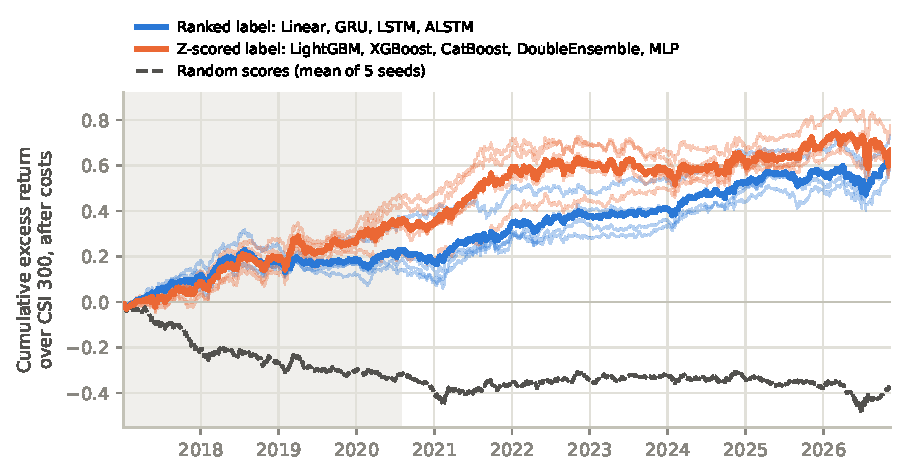
\includegraphics[width=\linewidth]{figures/cumulative_excess.pdf}
\caption{Cumulative excess return over the CSI\,300 after costs of the TopK-Dropout strategy for each model's seed ensemble, published protocol, grouped and coloured as in Figure~\ref{fig:rolling}. Dashed: the same strategy on random scores, mean of five seeds.}\label{fig:cum}
\end{figure}

\begin{table}[t]
\centering\small
\caption{TopK-Dropout portfolios of the seed ensembles: annualised excess return over the CSI\,300 after costs (\%) and information ratio. Published protocol in the first two windows; refit protocol in the recent window.}\label{tab:portfolio}
\begin{tabular}{lrrrrrr}
\toprule
 & \multicolumn{2}{c}{2017--07/2020} & \multicolumn{2}{c}{08/2020--2026} & \multicolumn{2}{c}{2023--2026, refit} \\
\cmidrule(lr){2-3}\cmidrule(lr){4-5}\cmidrule(lr){6-7}
Model & Return & IR & Return & IR & Return & IR \\
\midrule
Linear & 9.9 & 1.31 & 5.8 & 0.69 & 7.3 & 0.82 \\
LightGBM & 12.4 & 1.41 & 2.2 & 0.21 & 4.1 & 0.43 \\
XGBoost & 9.4 & 1.01 & 4.2 & 0.37 & 7.3 & 0.76 \\
CatBoost & 8.9 & 0.95 & 4.6 & 0.40 & 7.8 & 0.75 \\
DoubleEnsemble & 11.5 & 1.33 & 5.1 & 0.51 & 8.1 & 0.91 \\
MLP & 5.6 & 0.73 & 6.7 & 0.78 & 7.9 & 0.92 \\
GRU & 5.0 & 0.70 & 6.9 & 0.86 & -0.0 & -0.00 \\
LSTM & 3.8 & 0.56 & 7.8 & 1.01 & -- & -- \\
ALSTM & 5.8 & 0.92 & 5.8 & 0.74 & 4.2 & 0.54 \\
\midrule
Random scores (5 seeds) & -8.8 & -1.30 & -0.9 & -0.14 & -0.9 & -0.15 \\
\bottomrule

\end{tabular}
\end{table}

Table~\ref{tab:portfolio} and Figure~\ref{fig:cum} translate the signals into the benchmark's portfolio.
Excess return over the CSI\,300 is not all prediction: an equally weighted book of 50 stocks rebalanced slowly carries a size tilt and pays costs whatever its scores.
We therefore also run the strategy on i.i.d.\ random scores (five seeds).
That null strategy lost \NullRetPub{} a year against the index in the published window, when large caps led, and \NullRetPost{} ($\pm$\NullRetSDPost{} across seeds) after it.
Measured against it, the models' average excess return falls from \AboveNullPub{} to \AboveNullPost{} a year, a decline of \AboveNullDrop{}, in line with the decline in Rank IC.
Most refitted models still earn a positive excess return on 2023--2026, but the null strategy's spread across seeds on that window, \NullRetSDRecent{}, is a reminder of how short the window is.
Counting each of the \DSRTrials{} (model, seed) runs of the published protocol as a trial, the best post-window strategy, \DSRBest{}, has an information ratio of \DSRIR{}; its probabilistic Sharpe ratio against zero is \DSRPSR{}, and its deflated Sharpe ratio, which asks whether it beats the best of \DSRTrials{} skill-less strategies, is \DSRValue{}, short of the usual 0.95.

\subsection{Which features died}

\begin{figure}[t]
\centering
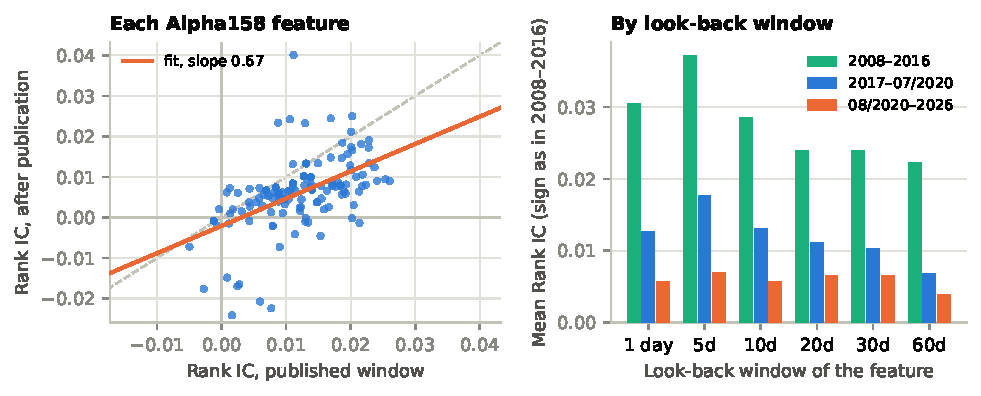
\includegraphics[width=\linewidth]{figures/feature_decay.pdf}
\caption{Left: daily Rank IC of each Alpha158 feature in the published window and after it, signed so that the 2008--2016 direction is positive; \FeatStrong{} features with a 2008--2016 Newey--West $|t|>3$. The dashed line is equality. Right: mean of the same quantity by look-back window and period.}\label{fig:features}
\end{figure}

The models only combine Alpha158 features, so the decay should be visible in the features themselves.
For the \FeatStrong{} of \FeatN{} features with a clear sign in 2008--2016, the mean Rank IC, signed in the 2008--2016 direction, is \FeatTrain{} in 2008--2016, \FeatPub{} in the published window and \FeatPost{} after it (Figure~\ref{fig:features}).
Two facts stand out.
First, the decline started before the published window: features lost \FeatDropTrainPub{} of their strength between 2008--2016 and 2017--2020, and another \FeatDropPubPost{} after.
Second, it is broad: the slope of post-window on published-window strength across features is \FeatSlope{}, the median ratio is \FeatMedianRatio{}, and \FeatFlips{} features changed sign.
The ``post-publication'' decline is therefore not something that started when the leaderboard was published; it is the continuation of a longer trend that the published window caught midway.

\section{Discussion}\label{sec:discussion}

\paragraph{What this does not show.}
Our split is a date, not an event.
The A-share market after 2020 differs from the market before it in many ways at once: a growing quantitative industry, a small-cap rally and its reversal, the quant drawdown of early 2024, and changes in trading rules and stamp duty.
We cannot say which of these, if any, caused the decay, and we do not claim that publishing the benchmark did.
The audit covers one universe, one feature set and one label; the backtest uses Qlib's simplified execution, with a single 9.5\% price-limit rule that is too strict for boards with 20\% limits; and we ran fewer seeds than the published table, two or three for the recurrent models under the published protocol and one under the refit protocol.

\paragraph{What it does show.}
A leaderboard computed on one 3.5-year window of a non-stationary market is an in-sample object.
Its level does not carry over, and its order carries over even less.
The differences between models are larger than seed noise, but inside the published window they are smaller than its sampling error, and after it they come in a different order.
Claims of a new state of the art on this benchmark should therefore come with (i) several seeds and a confidence set rather than a single best number, (ii) a second, later test window, (iii) a refit protocol, so that a reader can tell a better model from a better-timed one, and (iv) the same preprocessing for every model compared, or an ablation of the difference: on this benchmark the label normalisation moves a model by more than the published differences between these models.
The same reasoning applies to any benchmark built on a single historical window, including the newer ones for LLM trading agents.

\paragraph{Extensions.}
The pipeline is market-agnostic; running it on U.S.\ data with delisted stocks (for example CRSP) would show whether the pattern is specific to the A-share market.
The recurrent and attention models could be run with more seeds on a GPU.

\section{Conclusion}
The Qlib Alpha158 leaderboard reproduces on independent data, but only inside the window it was computed on.
Six years later the models keep a small, statistically positive signal, most of the published performance is gone, and the ranking between them has changed, largely along a preprocessing choice that the table does not report.
Code, configuration files, results and figures are at \url{https://github.com/Pearmaleka/qlib-oos-audit}.

\bibliographystyle{plainnat}
\bibliography{refs}

\appendix
\section{Rank IC by year}

\begin{table}[h]
\centering\small
\caption{Mean daily Rank IC by calendar year, published protocol, seed ensembles. 2017--2019 and the first seven months of 2020 form the published window; 2026 runs to 11 November.}\label{tab:yearly}
\setlength{\tabcolsep}{4pt}
\begin{tabular}{lrrrrrrrrr}
\toprule
Year & Linear & LightGBM & XGBoost & CatBoost & DoubleEnsemble & MLP & GRU & LSTM & ALSTM \\
\midrule
2017 & 0.073 & 0.074 & 0.074 & 0.069 & 0.073 & 0.069 & 0.066 & 0.067 & 0.071 \\
2018 & 0.047 & 0.052 & 0.053 & 0.048 & 0.056 & 0.044 & 0.043 & 0.051 & 0.041 \\
2019 & 0.030 & 0.035 & 0.037 & 0.029 & 0.036 & 0.032 & 0.029 & 0.034 & 0.035 \\
2020 & 0.038 & 0.036 & 0.040 & 0.037 & 0.038 & 0.028 & 0.031 & 0.028 & 0.037 \\
2021 & 0.022 & 0.025 & 0.024 & 0.022 & 0.027 & 0.025 & 0.029 & 0.037 & 0.034 \\
2022 & 0.016 & 0.011 & 0.010 & 0.011 & 0.011 & 0.016 & 0.030 & 0.038 & 0.037 \\
2023 & 0.013 & 0.002 & 0.001 & -0.006 & 0.003 & 0.010 & 0.015 & 0.024 & 0.023 \\
2024 & 0.018 & 0.016 & 0.012 & 0.006 & 0.015 & 0.011 & 0.032 & 0.035 & 0.037 \\
2025 & 0.025 & 0.012 & 0.014 & 0.009 & 0.013 & 0.007 & 0.028 & 0.033 & 0.026 \\
2026 & 0.012 & 0.019 & 0.015 & 0.009 & 0.019 & 0.018 & 0.033 & 0.043 & 0.041 \\
\bottomrule
\end{tabular}

\end{table}

\end{document}
